% =====================================================================
% 1. INTRODUCTION            target: 1.5 - 2 pages
%
% Goal of this section: a young researcher who has never worked on time
% series should be able to read it and understand WHY this work exists
% and WHAT I added. No maths here, no experimental detail.
% =====================================================================

\section{Introduction}
\label{sec:intro}

\begin{guide}
Five short paragraphs, then a bullet list of contributions. Keep every sentence
short. Explain any term the first time it appears.
\begin{itemize}\itemsep2pt
  \item \textbf{P1 -- the setting.} What is a time series and where does time series
        classification (TSC) matter? Give two or three everyday examples (web traffic,
        heartbeats, machine sensors).
  \item \textbf{P2 -- the gap.} Modern deep models are black boxes. Why is that a real
        problem (trust, debugging, regulation, wrong reasons for a right answer)?
  \item \textbf{P3 -- the two families of answers.} Post-hoc explainers (SHAP, LIME,
        saliency) versus models that explain themselves. Say briefly why the second
        is preferable here.
  \item \textbf{P4 -- the starting point.} \millet{} \citep{early2024millet}: MIL
        pooling gives an explanation for free. State clearly that this is
        \emph{existing} work, and that it is where I started.
  \item \textbf{P5 -- my angle.} What I noticed was missing or weak, and what I did
        about it, in three or four sentences. This paragraph is the bridge to the
        contribution list.
\end{itemize}
\textbf{Questions to answer:} Why should anyone care about a \emph{smaller} model?
What was unsatisfying in the baseline explanation quality? What did I want to be true
at the end of the internship that was not true at the start?
\end{guide}

\subsection*{Motivation}


{We are facing on daily basis the Time Series problems in our real life like in hospital the doctor see the heartbeat of the patient, in the industry the machine sensors are used to monitor the machine health and in the web traffic the web traffic is monitored to see the user behaviour. The time series data is everywhere and it is important to classify them correctly.}

{Modern deep models are black boxes first their problems is they cannot explane the reason of their answer like they are predicting specific class then they should know the reason of it.}

{For Explanation of deep model there are alot of others techniques like SHAP,LIME , Saliency but thee issue with them they will execute after we will get the model prediction and these are also taking so much time to execute and they are not giving the correct reason of the prediction. So it is better to have a model which can explain itself.
(cite \citep{ribeiro2016lime, lundberg2017shap, rudin2019stop}).}

{So for the basline we select  \millet{} as the starting point \citep{early2024millet}. where we get free explanation the problem was that we were getting the decent explanation of model but it the size of model itself was large with 424k parameters so in MCU application  it is hard to integrate because when we see the base line that is 38.6k parameters this is good is this range as they "MLPerf Tiny Benchmark" mention in their paper and they are getting 92 percent accuracy after quantixation (it is a technique to reduce the size) with hurting the accuracy and the thing was they didnot have intrepretation part that i will explain in this repot .}

{ So what i observe from these research from millet paper they have classiification + interpretabilty with with big size and for MLPerf Tiny Benchmark they have small size micro model for only give us classification prediction soI try yto solve both things together in one model we try different encoder with pooling techniques and finallly we got seanet model that size is 45K   param before quantizattion and plus also giving the better explanation of the model will be best for the MCU application}

% ---------------------------------------------------------------------
% Optional: one small "teaser" figure. Very effective on page 1.
% Idea: the same time series with (a) a black-box label only, and
% (b) the same label plus a per-time-step importance curve.
% ---------------------------------------------------------------------
\begin{figure}[t]
  \centering
  
 % ...existing code...
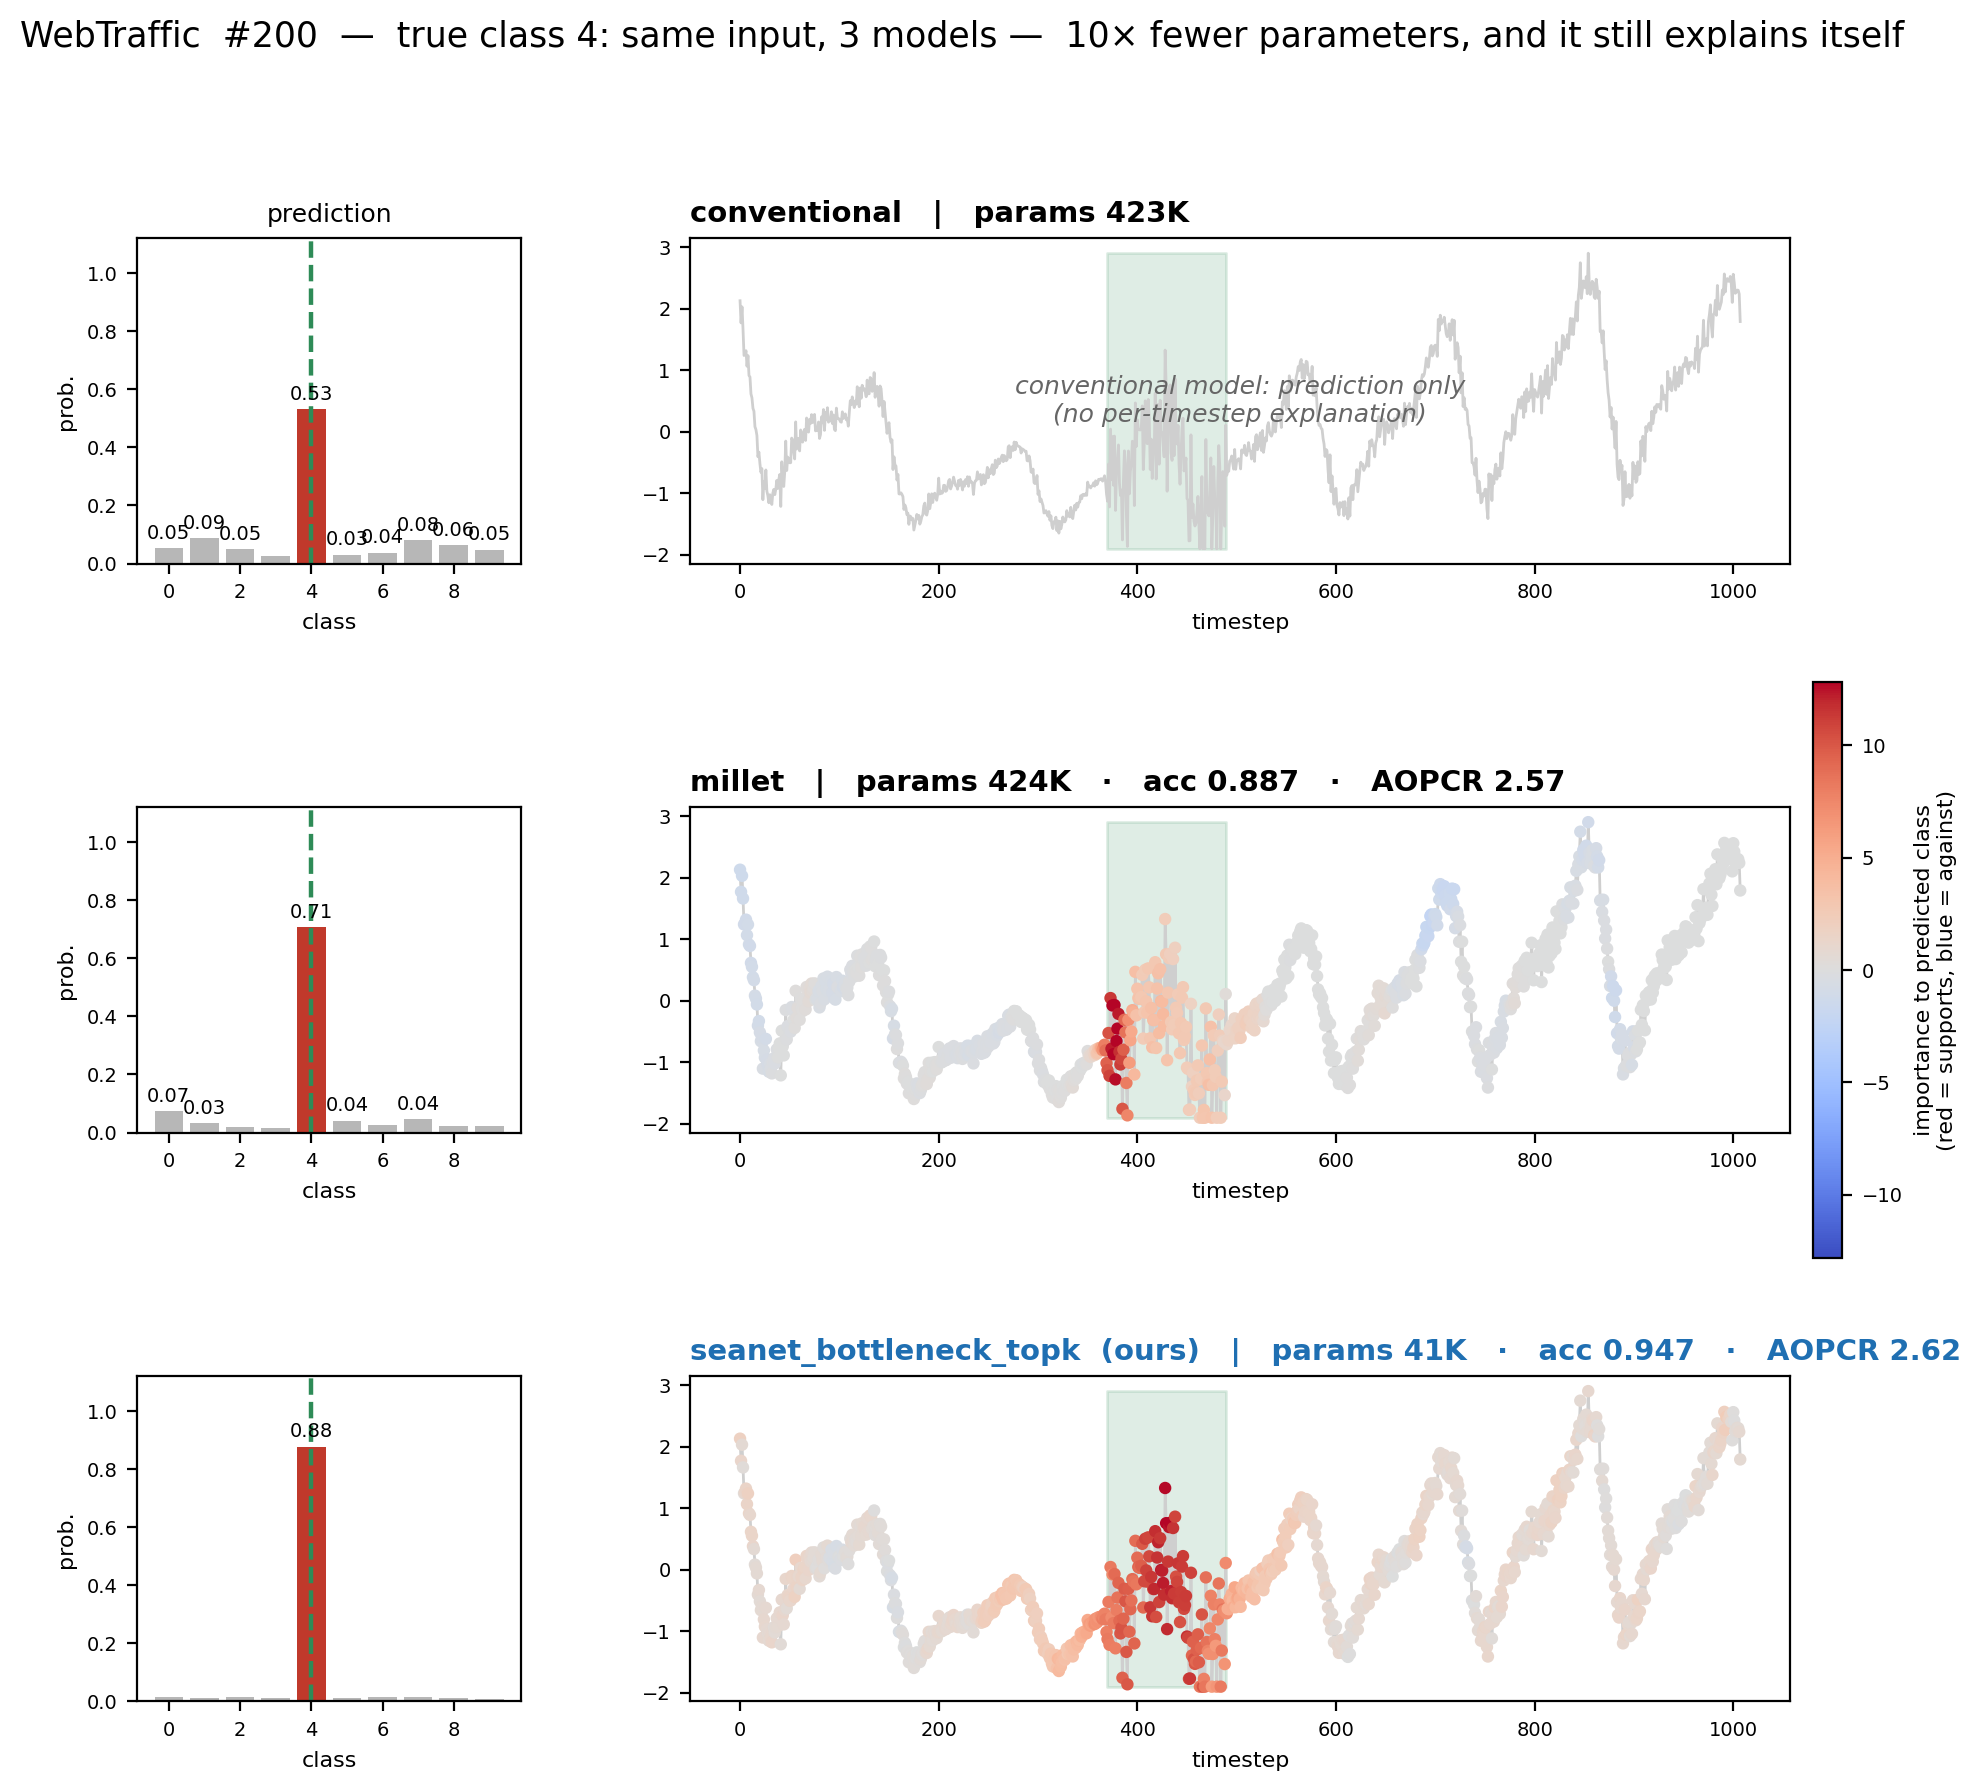
\includegraphics[width=0.85\linewidth]{results/SEA_NET/teaser/2026-08-06_15-02-34/teaser_WebTraffic_idx0200.png}
% ...existing code...
  \caption{\todo{Caption: a self-explaining classifier does not only say
  \emph{which} class, it says \emph{where} in the series the evidence is.}}
  \label{fig:teaser}
\end{figure}

\subsection*{Contributions}

\begin{guide}
This list is the most important part of the whole report for the examiner. Rules:
\begin{itemize}\itemsep2pt
  \item Use \textbf{``I''} here. This is my personal work.
  \item Each bullet = one thing I built or found, plus the evidence (a section or
        table number), not a promise.
  \item Do not list things that already existed. Those belong in
        \Cref{sec:background}.
  \item Four to six bullets is the right size.
\end{itemize}
\textbf{Questions to answer:} If my supervisor had to name my three deliverables in
one sentence each, what would they be? Which of them did nobody ask me for (the
initiative I took myself)?
\end{guide}

\begin{contribution}
The work described in this report is my own, unless a paragraph is explicitly
marked as existing work. My main contributions are:
\begin{itemize}\itemsep3pt
  \item \textbf{The \seanet{} encoder family.}
  I designed compact encoders for feature extraction using TCN variants:
  depthwise-separable convolution, bottleneck, gated and input-gated blocks,
  spike/trend branches, multi-scale channels, and pyramid structures
  (\Cref{sec:architecture}).

  \item \textbf{Seven new MIL pooling heads.}
  I developed improved pooling heads inspired by conjunctive pooling:
  \texttt{classwise\_conjunctive},
  \texttt{softmax\_conjunctive},
  \texttt{adaptive\_classwise\_topk\_conjunctive},
  \texttt{attention\_max},
  \texttt{gated\_attention},
  and \texttt{dualstream\_conjunctive}.
  Each targets a weakness of \millet{} conjunctive pooling
  (\Cref{sec:pooling}).

  \item \textbf{A modular, config-driven benchmark.}
  {I create a config files it will works as a pipe lines just change the config files settings we will get different results like we can get optuna fine tune on pair of encoder and pooling get the best parameters then use that for final traning and also use MLflow the track the experiments so our contribution here I provided the template so any kind of encoder or pooling module will integrate the whole pipeline easily with less efforts. }
\end{itemize}
\end{contribution}

\subsection*{Structure of this report}

\begin{guide}
Six or seven lines, one per section, so the reader can skip straight to what they
want. Write this at the very end, when the section numbers are stable.
\end{guide}

\todo{One short paragraph mapping the report:
\Cref{sec:context} the context of the internship,
\Cref{sec:objectives} the mission I was given,
\Cref{sec:background} the background a non-specialist needs,
\Cref{sec:architecture} and \Cref{sec:pooling} my proposed model,
\Cref{sec:setup} how I ran the experiments,
\Cref{sec:results} and \Cref{sec:discussion} what came out of them,
\Cref{sec:skills} the skills I gained,
\Cref{sec:conclusion} the conclusion, and the appendix the additional results.}
